\documentclass{article}
\usepackage{graphicx} % Required for inserting images
\usepackage{float}
\usepackage{caption}
\usepackage{listings}
\usepackage{geometry}

\geometry{left=1.8cm, top=1cm, right=1.8cm, bottom=1cm, footskip=.5cm}



\title{Parallel and Distributed Computing - First Project Report \\ FEUP 24/25 - 2nd Semester} 

\author{
Turma 07 Grupo 11 \\
Carlos Sanches, up202107694 \\
João Rebelo, up202107209 \\
Luís Ganço, up202004196
}
\date{March 21, 2025}

\begin{document}

\newpage 
\vspace{0.in}

\maketitle
\begin{center}
    \large \textit{Project Theme:} Performance Comparison of Single-Core and Multi-Core Systems
\end{center}
\vspace{1.3in}
% Add the table of contents (index)
\tableofcontents
\newpage % Start a new page after the table of contents

\section{Introduction}

In modern computing, the performance of processors is heavily influenced by the memory hierarchy, particularly when handling large datasets. Matrix multiplication, a fundamental operation in many scientific and engineering applications, serves as a case study to explore these performance dynamics. This project aims to evaluate the impact of memory hierarchy on processor performance by implementing and analyzing different versions of matrix multiplication algorithms in multiple programming languages.

The project is divided into two main parts: single-core and multi-core performance evaluations. In single-core evaluation, we implement and compare matrix multiplication algorithms in C/C++ with Java. We measure processing times for matrices of varying sizes and analyze the effects of different algorithmic approaches, including a block-oriented implementation. The Performance API (PAPI) is utilized to collect relevant performance metrics, such as cache misses and floating-point operations, to provide deeper insights into the behavior of the memory hierarchy.

For the multi-core evaluation, we parallelize the matrix multiplication algorithms using OpenMP and analyze their performance in terms of MFlops, speedup, and efficiency. Two parallelization strategies are explored, and their results are compared to understand the trade-offs between different parallel implementations.

This report documents the implementation details, performance metrics, and analysis of the results obtained from both single-core and multi-core evaluations. 

\section{Algorithms Explanation}

\subsection{Single-Core Algorithms}

\subsubsection{Naive Matrix Multiplication}

\begin{itemize}
\item Element-wise multiplication and summation: Each element of a row is multiplied by the corresponding element of a column, and all of them are summed up;
\item Time complexity: $O(n^3)$, as the algorithm has three nested loops.
\end{itemize}

\subsubsection{Line-by-Line Matrix Multiplication}

\begin{itemize}
\item In this variant, the multiplication is performed by iterating over the rows of the first matrix and the columns of the second matrix;
\item For each row in the first matrix, the algorithm multiplies the row by each column in the second matrix, summing the results to produce the corresponding element in the result matrix;
\item This approach improves cache locality compared to the naive element-wise multiplication, as it accesses the elements of the second matrix in a more sequential manner;
\item Time complexity: $O(n^3)$, as it still involves three nested loops, but with a different order of iteration.
\end{itemize}

\subsubsection{Block-Oriented Matrix Multiplication}

\begin{itemize}
\item The block-oriented approach divides the matrices into smaller submatrices (blocks) and performs multiplication on these blocks;
\item The algorithm iterates over the blocks of the matrices, multiplying corresponding blocks and accumulating the results;
\item This approach is particularly useful for large matrices, as it improves cache efficiency by operating on smaller blocks that fit into the cache;
\item The block size should be chosen carefully to balance cache utilization and overhead. Common block sizes are 128, 256, or 512, depending on the cache size of the system;
\item Time complexity: $O(n^3)$, as the overall number of operations remains the same, but the block size affects the performance due to cache effects.
\end{itemize}

\subsection{Multi-Core Algorithms}

The parallel implementation uses OpenMP to distribute the workload across multiple CPU cores. Two variants were implemented:


\subsubsection{Outer Loop Parallelization}


\begin{itemize}
\item The outermost loop is parallelized using OpenMP's \textbf{\lstinline{#pragma omp parallel for}} directive;
\item This approach divides the rows of the first matrix among the available threads;
\item Each thread computes a portion of the result matrix by iterating over its assigned rows;
\item This method is effective for large matrices, as it reduces the workload per thread and improves scalability.
\end{itemize}

\subsubsection{Inner Loop Parallelization}
        
\begin{itemize}
\item The innermost loop is parallelized using OpenMP's \textbf{\lstinline{#pragma omp parallel for}} directive;
\item This approach divides the columns of the second matrix among the available threads;
\item Each thread computes a portion of the result matrix by iterating over its assigned columns;
\item This method can improve cache utilization, as threads work on smaller portions of the matrix.
\end{itemize}


\section{Performance Metrics}

We decided to use the following metrics to evaluate performance:

\begin{itemize}
    \item \textbf{Execution Time - } Measures the total time taken to complete matrix multiplication for different matrix sizes. This metric provides a straightforward way to compare the overall efficiency of the implementations in C++ and Java.
    
    \item \textbf{Data Cache Misses (DCM) - } Tracks the number of times data requested by the CPU are not found in the cache, requiring slower memory access. We analyze both L1 and L2 cache misses to better understand how memory access patterns impact performance, especially for larger matrix sizes. Specifically, we use the following PAPI events:
    \begin{itemize}
        \item \textbf{L1 Data Cache Misses (PAPI\_L1\_DCM)}: Measures the number of Level 1 data cache misses.
        \item \textbf{L2 Data Cache Misses (PAPI\_L2\_DCM)}: Measures the number of Level 2 data cache misses.
    \end{itemize}

    \item \textbf{Floating-Point Operations (PAPI\_FP\_OPS) - } Measures the number of floating-point operations performed during matrix multiplication. This metric helps us evaluate the computational intensity of the algorithm and its efficiency in utilizing the CPU's floating-point units.

    \item \textbf{Total Instructions (PAPI\_TOT\_INS) - } Measures the total number of instructions executed during matrix multiplication. This metric provides insight into the overall workload and how efficiently the CPU processes the instructions.

    \item \textbf{GFlops - } Measures the number of floating-point operations per second, reflecting the raw computational throughput. Although the assignment description mentions MFlops, we will use GFlops for our performance evaluation, as it provides a cleaner and more intuitive representation of performance, especially for larger matrices and higher-performance systems. Since 1 GFlops equals 1000 MFlops, this change in unit does not affect the underlying metric, but simplifies the visualization of results.
\end{itemize}

This combination of metrics allowed us to assess not only how fast the algorithms run but also how efficiently they utilize the hardware, considering both computation and memory access patterns.

\section{Results and Analysis}

\textbf{Note:} The following results were obtained using an AMD Ryzen 7 7730U processor and Linux as the operating system (Ubuntu 24.04).

\subsection{Single-Core}

\subsubsection{Naive Matrix Multiplication}

\begin{table}[H]
\centering
\caption*{\textbf{ Table 1: C++ Performance Results}}
\begin{tabular}{||c | c | c | c | c||} 
 \hline
 \textbf{Dimensions} & \textbf{Execution Time (s)} & \textbf{GFlops} & \textbf{L1 DCM} & \textbf{L2 DCM} \\  
 \hline \hline
 600x600  & 0.154   & 2.80   & 241678983   & 448582    \\  
 \hline
 1000x1000 & 0.702   & 2.85   & 1136969844 & 3488117  \\  
 \hline
 1400x1400 & 2.846   & 1.93   & 3125017136 & 58169452 \\  
 \hline
 1800x1800 & 6.711   & 1.74   & 7059740261 & 94416650 \\  
 \hline
 2200x2200 & 16.870  & 1.26   & 15939144633 & 558295715 \\  
 \hline
 2600x2600 & 41.912  & 0.84   & 30910168160 & 2305966036 \\  
 \hline
 3000x3000 & 67.189  & 0.80   & 50421145206 & 6043903995 \\  
 \hline
\end{tabular}
\end{table}

\begin{table}[H]
\centering
\caption*{\textbf{ Table 2: Java Performance Results}}
\begin{tabular}{||c | c | c||} 
 \hline
 \textbf{Dimensions} & \textbf{Execution Time (s)} & \textbf{GFlops} \\  
 \hline \hline
 600x600  & 0.254   & 1.70   \\  
 \hline
 1000x1000 & 1.581   & 1.27   \\  
 \hline
 1400x1400 & 8.502   & 0.65   \\  
 \hline
 1800x1800 & 23.912  & 0.49   \\  
 \hline
 2200x2200 & 51.042  & 0.42   \\  
 \hline
 2600x2600 & 104.170 & 0.34   \\  
 \hline
 3000x3000 & 175.885 & 0.31   \\  
 \hline
\end{tabular}
\end{table}

After comparing the performance results of C++ and Java, it is clear that C++ is faster. To confirm this, we plot relevant graphs that compare the performance metrics of both languages, as shown below.

\begin{figure}[H]
    \centering
    \begin{minipage}{0.32\textwidth}
        \centering
        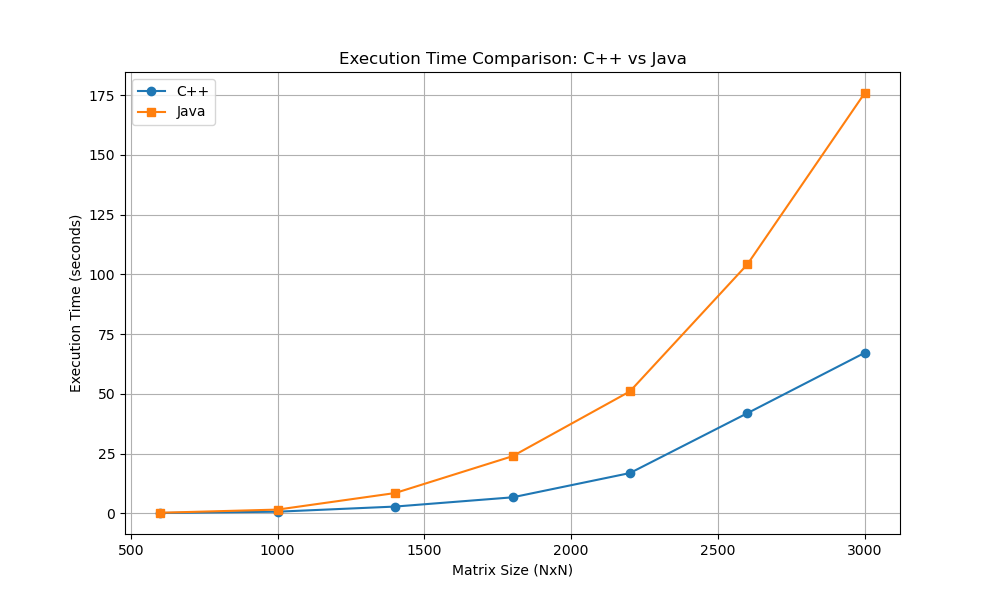
\includegraphics[width=\textwidth]{Figure_1.png}
        \caption{\small Execution Time Comparison}
        \label{fig:execution_time}
    \end{minipage}
    \hfill
    \begin{minipage}{0.32\textwidth}
        \centering
        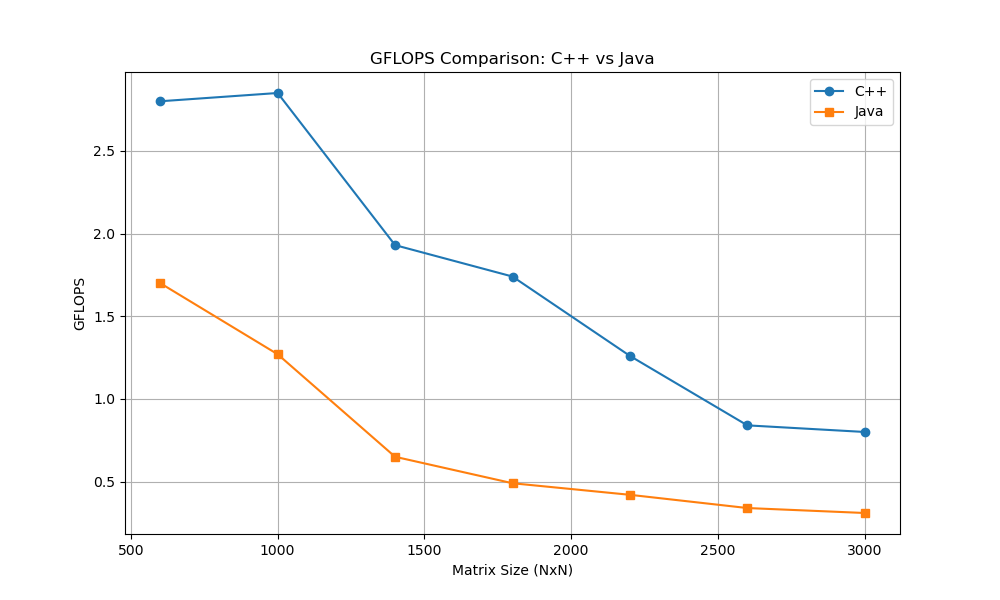
\includegraphics[width=\textwidth]{Figure_2.png}
        \caption{\small Line-by-Line GFlops Comparison}
        \label{fig:flops}
    \end{minipage}
    \hfill
    \begin{minipage}{0.32\textwidth}
        \centering
        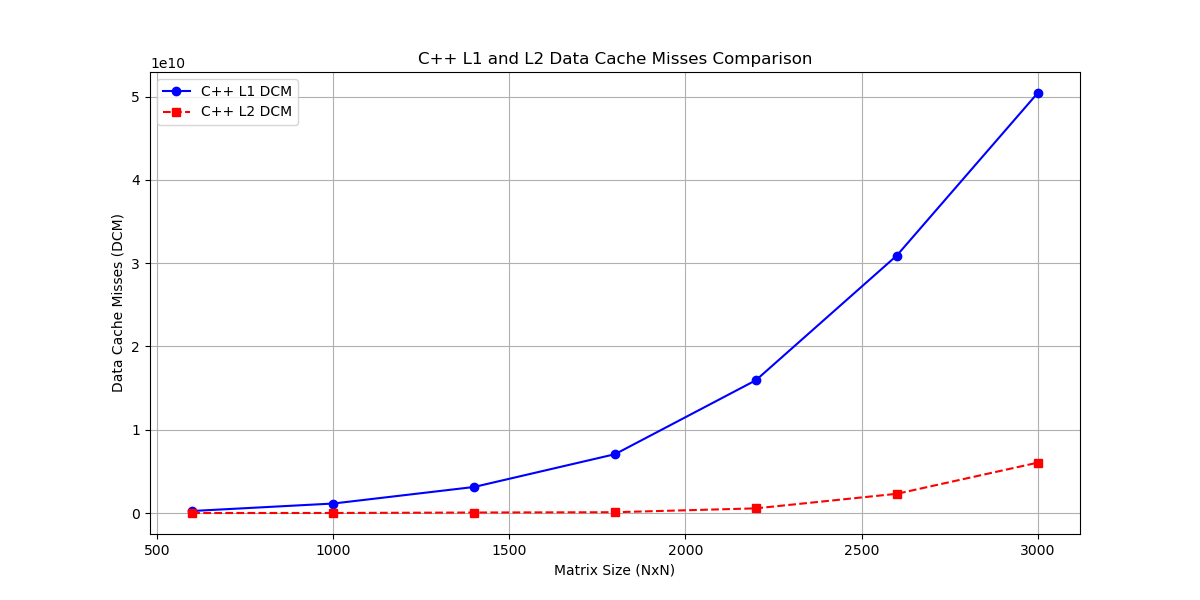
\includegraphics[width=\textwidth]{Figure_3.png}
        \caption{\small C++ DCM Comparison}
        \label{fig:cache_misses}
    \end{minipage}
\end{figure}

Figure 1 supports our initial observation, while Figures 2 and 3 provide valuable insight into the underlying factors that affect performance.

\begin{itemize}
    \item C++ outperforms Java consistently across all matrix sizes, with higher GFlops values;
    \item As the matrix size grows, performance (GFlops) decreases for both languages, but the drop is sharper for Java;
    \item This shows that C++ handles large matrix multiplications more efficiently, likely due to better memory management and lower runtime overhead;
    \item L1 cache misses grow exponentially as matrix size increases, indicating that larger matrices don't fit well in the smaller, faster L1 cache;
    \item L2 cache misses are much lower, but they still increase gradually, highlighting that more data spills into higher cache levels;
    \item This pattern suggests that performance degradation for larger matrices is tied to cache inefficiencies, with more memory accesses going to slower cache layers or RAM.
\end{itemize}

\subsubsection{Line-by-Line Matrix Multiplication}

\begin{table}[H]
\centering
\caption*{\textbf{ Table 3: C++ Line-by-Line Performance Results}}

\begin{tabular}{||c | c | c | c | c||} 
 \hline
 \textbf{Dimensions} & \textbf{Execution Time (s)} & \textbf{GFlops} & \textbf{L1 DCM} & \textbf{L2 DCM} \\  
 \hline \hline
 600x600  & 0.109   & 3.96   & 27610902   & 197852    \\  
 \hline
 1000x1000 & 0.474   & 4.22   & 128270508 & 958787  \\  
 \hline
 1400x1400 & 1.487   & 3.69   & 356961253 & 4028340 \\  
 \hline
 1800x1800 & 3.175   & 3.67   & 772784793 & 9800958 \\  
 \hline
 2200x2200 & 5.891   & 3.61   & 2014640122 & 4182780 \\  
 \hline
 2600x2600 & 9.736   & 3.61   & 4294621566 & 6984457 \\  
 \hline
 3000x3000 & 14.951  & 3.61   & 6698316610 & 10414106 \\  
 \hline
\end{tabular}
\end{table}

\begin{table}[H]
\centering
\caption*{\textbf{ Table 4: Java Line-by-Line Performance Results}}
\begin{tabular}{||c | c | c||} 
 \hline
 \textbf{Dimensions} & \textbf{Execution Time (s)} & \textbf{GFlops} \\  
 \hline \hline
 600x600  & 0.091   & 4.75   \\  
 \hline
 1000x1000 & 0.399   & 5.01   \\  
 \hline
 1400x1400 & 1.342   & 4.09   \\  
 \hline
 1800x1800 & 2.947   & 3.96   \\  
 \hline
 2200x2200 & 5.505   & 3.87   \\  
 \hline
 2600x2600 & 10.947  & 3.21   \\  
 \hline
 3000x3000 & 16.040  & 3.37   \\  
 \hline
\end{tabular}
\end{table}

After analyzing the performance results of C++ and Java for line-by-line matrix multiplication, Java achieves better execution times and higher GFLOPS for smaller matrices, while C++ demonstrates more consistent performance as the matrix size grows. To validate these findings, we have plotted relevant graphs comparing the performance metrics of both languages, as illustrated below.

\begin{figure}[H]
    \centering
    \begin{minipage}{0.32\textwidth}
        \centering
        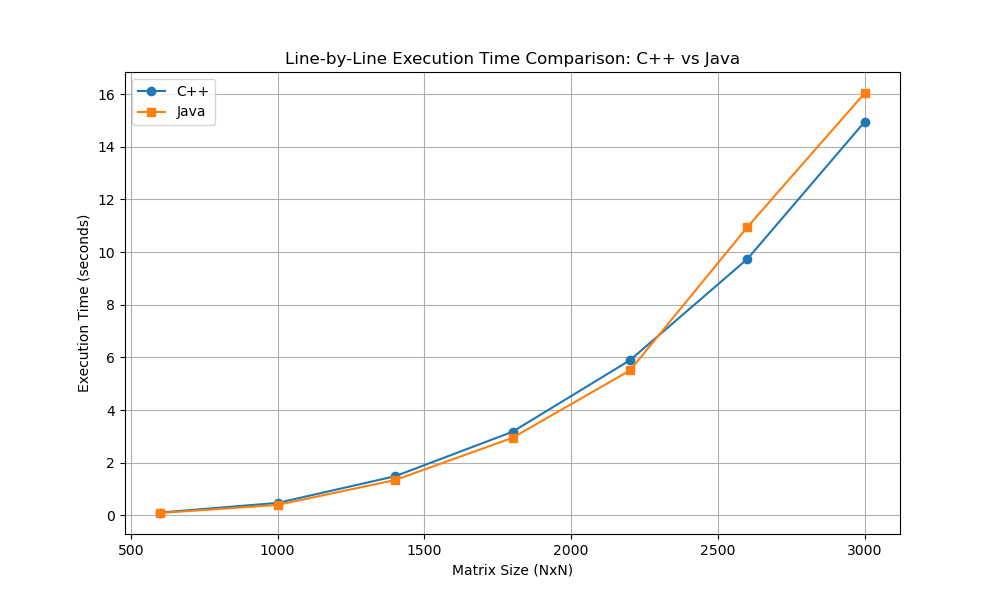
\includegraphics[width=\textwidth]{Figure_4.png}
        \caption{\small Line-by-Line Execution Time Comparison}
        \label{fig:execution_time_linebyline}
    \end{minipage}
    \hfill
    \begin{minipage}{0.32\textwidth}
        \centering
        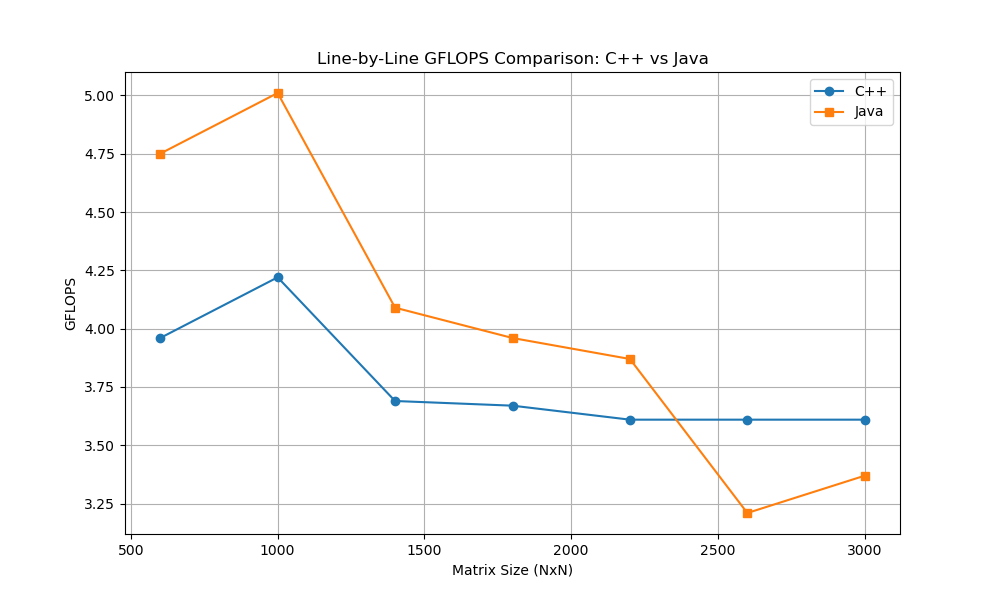
\includegraphics[width=\textwidth]{Figure_5.png}
        \caption{\small Line-by-Line GFlops Comparison}
        \label{fig:flops_linebyline}
    \end{minipage}
    \hfill
    \begin{minipage}{0.32\textwidth}
        \centering
        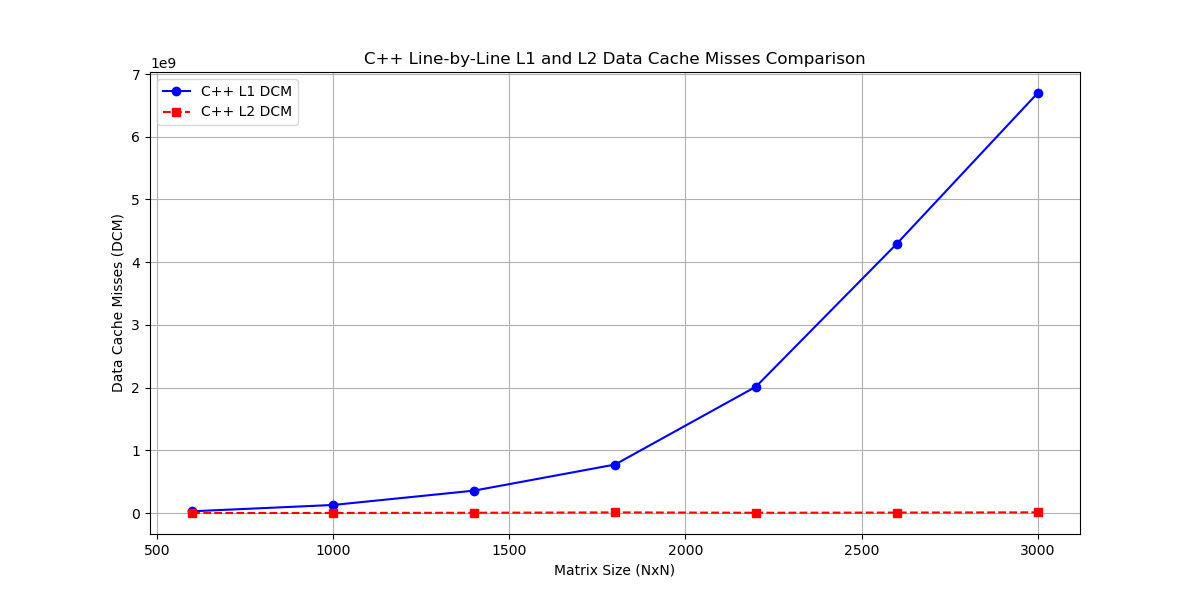
\includegraphics[width=\textwidth]{Figure_6.png}
        \caption{\small C++ DCM Comparison}
        \label{fig:cache_misses_linebyline}
    \end{minipage}
\end{figure}


Additionally, it was asked to register the processing time from 4096x4096 to 10240x10240 with intervals of 2048 in the C++ version:

\begin{table}[H]
\centering

\caption*{\textbf{Table 5: C++ Line-by-Line Bigger Matrices Performance Results}}
\begin{tabular}{||c | c | c | c | c||} 
 \hline
 \textbf{Dimensions} & \textbf{Execution Time (s)} & \textbf{GFlops} & \textbf{L1 DCM} & \textbf{L2 DCM} \\  
 \hline \hline
 4096x4096  & 38.332   & 3.59   & 17281550488   & 26563644    \\  
 \hline
 6144x6144  & 131.659  & 3.52   & 58311966805   & 89317155    \\  
 \hline
 8192x8192  & 313.217  & 3.51   & 138166449164  & 204171358   \\  
 \hline
 10240x10240 & 623.608  & 3.44   & 269797217196  & 502826446   \\  
 \hline
\end{tabular}
\end{table}

For line-by-line multiplication:

\begin{itemize}
    \item C++ is more efficient for large matrix computations, maintaining consistent performance (around 3.6-3.9 GFLOPS) as matrix size increases, thanks to better memory management and lower runtime overhead.
    \item Java performs well for small matrices, achieving higher GFLOPS (e.g., 4.75 GFLOPS at 600x600) due to effective JIT optimization, but its performance degrades significantly as the matrix size grows, likely due to higher memory overhead and garbage collection;
    \item Cache performance is a key factor in execution time, as a higher number of cache misses leads to increased memory access delays. When a cache miss occurs, the processor must retrieve data from slower/lower cache layers or main memory, consuming extra clock cycles. Additionally, Java's performance is further impacted by its runtime overhead, including Just-In-Time (JIT) compilation and garbage collection.
\end{itemize}

\subsubsection{Block-Oriented Matrix Multiplication}

\begin{table}[H]
\centering
\caption*{\textbf{Table 6: C++ Block Multiplication Performance Results (Block Sizes: 128, 256, 512)}}
\begin{tabular}{||c | c | c | c | c | c||} 
 \hline
 \textbf{Block Size} & \textbf{Dimensions} & \textbf{Execution Time (s)} & \textbf{GFlops} & \textbf{L1 DCM} & \textbf{L2 DCM} \\  
 \hline \hline
 128  & 4096x4096  & 165.188  & 0.83  & 72724290894   & 51805287    \\  
 \hline
 128  & 6144x6144  & 599.105  & 0.77  & 254882822662  & 193298357   \\  
 \hline
 128  & 8192x8192  & -        & -     & -             & -           \\  
 \hline
 128  & 10240x10240 & -       & -     & -             & -           \\  
 \hline \hline
 256  & 4096x4096  & 167.468  & 0.82  & 72029153308   & 897392949   \\  
 \hline
 256  & 6144x6144  & 572.747  & 0.81  & 247672155393  & 3195262285  \\  
 \hline
 256  & 8192x8192  & 1335.049 & 0.82  & 576990897213  & 11366549854 \\  
 \hline
 256  & 10240x10240 & 2727.813 & 0.79  & 1172701454549 & 25526270656 \\  
 \hline \hline
 512  & 4096x4096  & 188.230  & 0.73  & 121210979798  & 3686113280  \\  
 \hline
 512  & 6144x6144  & 561.051  & 0.83  & 247393755023  & 5869301468  \\  
 \hline
 512  & 8192x8192  & -        & -     & -             & -           \\  
 \hline
 512  & 10240x10240 & -       & -     & -             & -           \\  
 \hline
\end{tabular}
\end{table}

\textbf{Note:} The "\textbf{-}" symbol indicates that the execution was canceled due to excessively long execution times.
\begin{itemize}
    \item Block multiplication shows poor scalability for large matrices (8192x8192 and 10240x10240);
    \item Execution times grow exponentially with matrix size, making it impractical for large-scale computations without optimization. For example, the executions for 8192x8192 and 10240x10240 with block sizes 128 and 512 were canceled due to excessively long execution times, which was sufficient to conclude that block multiplication is computationally expensive for very large matrices;
    \item The GFlops values are consistently low (around 0.7–0.8 GFLOPS), indicating suboptimal performance. This suggests that this implementation does not effectively utilize the hardware's computational capabilities;
    \item L1 and L2 Data Cache Misses (DCM) increase significantly with larger matrices, indicating poor cache utilization. This highlights the need for better memory access patterns to reduce cache misses and improve performance.
\end{itemize}

\subsection{Multi-Core}

\begin{table}[H]
\centering
\caption*{\textbf{Table 7: C++ Line-by-Line Performance Results (Outer Loop Parallelization)}}
\begin{tabular}{||c | c | c | c | c | c||} 
 \hline
 \textbf{Dimensions} & \textbf{Execution Time (s)} & \textbf{L1 DCM} & \textbf{L2 DCM} & \textbf{FP OPS} & \textbf{TOT INS} \\  
 \hline \hline
 600x600  & 0.027   & 1924091   & 17330   & 27360001   & 113622169    \\  
 \hline
 1000x1000 & 0.116   & 9370417   & 60217   & 126000001   & 511795717  \\  
 \hline
 1400x1400 & 0.277   & 41090728   & 104111   & 344960001   & 1392538475 \\  
 \hline
 1800x1800 & 0.528   & 90382230   & 149096   & 732240001   & 2949387953 \\  
 \hline
 2200x2200 & 1.131   & 167081583   & 236023   & 1335840001   & 5372806495 \\  
 \hline
 2600x2600 & 2.086   & 280300693   & 555219   & 2203760001   & 8855308697 \\  
 \hline
 3000x3000 & 3.559   & 429083491   & 898157   & 3384000001   & 13588892279 \\  
 \hline
 4096x4096 & 8.299   & 1091464928   & 2332638   & 8589934593   & 34454331821 \\  
 \hline
 6144x6144 & 30.345   & 3683033942   & 9221214   & 28991029286   & 116178953875 \\  
 \hline
 8192x8192 & 73.170   & 8723285628   & 27789743   & 68719476737   & 275258134329 \\  
 \hline
 10240x10240 & 216.851   & 16994047992   & 131991061   & 134217736591   & 537461781358 \\  
 \hline
\end{tabular}
\end{table}

\begin{table}[H]
\centering
\caption*{\textbf{Table 8: C++ Line-by-Line Performance Results (Inner Loop Parallelization)}}
\begin{tabular}{||c | c | c | c | c | c||} 
 \hline
 \textbf{Dimensions} & \textbf{Execution Time (s)} & \textbf{L1 DCM} & \textbf{L2 DCM} & \textbf{FP OPS} & \textbf{TOT INS} \\  
 \hline \hline
 600x600  & 0.170   & 4303194   & 2220916   & 27360001   & 176516701    \\  
 \hline
 1000x1000 & 0.458   & 19228602   & 5246945   & 126000001   & 622628615  \\  
 \hline
 1400x1400 & 1.340   & 47916291   & 13397481   & 344960001   & 1649689186 \\  
 \hline
 1800x1800 & 2.950   & 93257787   & 34408060   & 732240001   & 3495964625 \\  
 \hline
 2200x2200 & 5.079   & 150167551   & 125759014   & 1335840001   & 6020016060 \\  
 \hline
 2600x2600 & 7.828   & 225078374   & 197407259   & 2203760001   & 9385227382 \\  
 \hline
 3000x3000 & 11.612   & 327859145   & 303356737   & 3384000001   & 14234349974 \\  
 \hline
 4096x4096 & 27.848   & 856407327   & 657927564   & 8589934593   & 35654285153 \\  
 \hline
 6144x6144 & 73.143   & 2636101874   & 1002581155   & 28991029249   & 116461371453 \\  
 \hline
 8192x8192 & 152.773   & 6077988446   & 1439078099   & 68719476737   & 269361045658 \\  
 \hline
 10240x10240 & 285.668   & 12285236091   & 1986263686   & 134217728001   & 514585201807 \\  
 \hline
\end{tabular}
\end{table}

Relevant plots:

\begin{figure}[H]
    \centering
    \begin{minipage}{0.48\textwidth} % First row, first image (additional image)
        \centering
        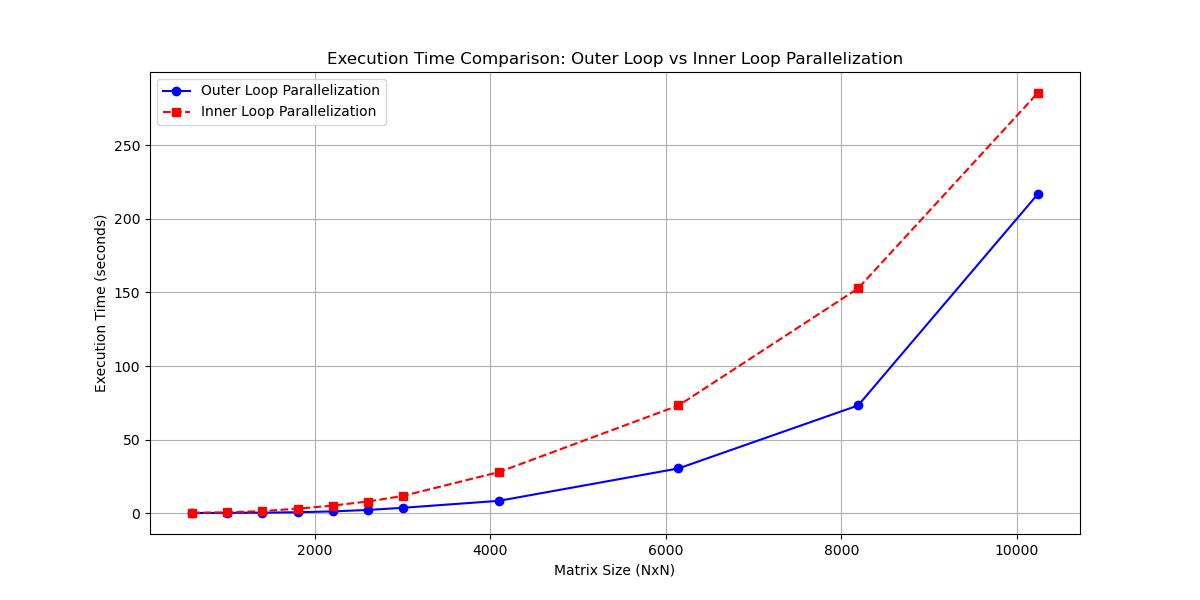
\includegraphics[width=\textwidth]{Figure_7.png} % Replace with your fifth image
        \caption{\small Parallel Execution Tine Comparison}
        \label{fig:execution_time_parallel}
    \end{minipage}
    \hfill
    \begin{minipage}{0.48\textwidth} % First row, second image
        \centering
        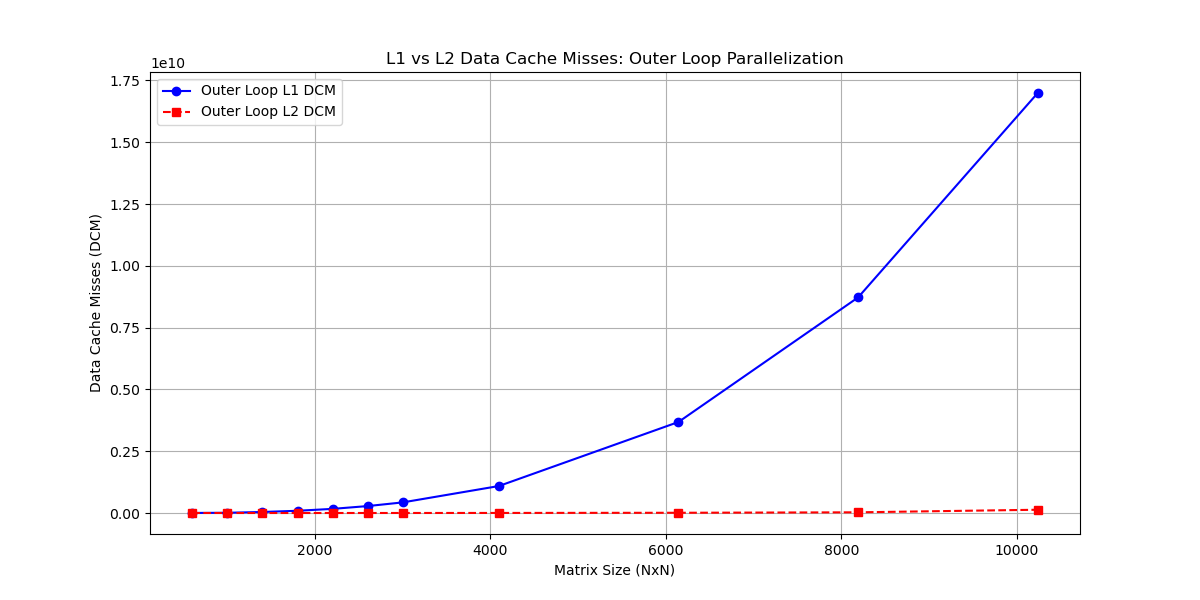
\includegraphics[width=\textwidth]{Figure_8.png} % Replace with your first image
        \caption{\small Outer Parallelization L1 vs L2 DCM Comparison}
        \label{fig:cache_misses_parallel1}
    \end{minipage}
    \vspace{0.5cm} % Add vertical space between rows

    \begin{minipage}{0.48\textwidth} % Second row, first image
        \centering
        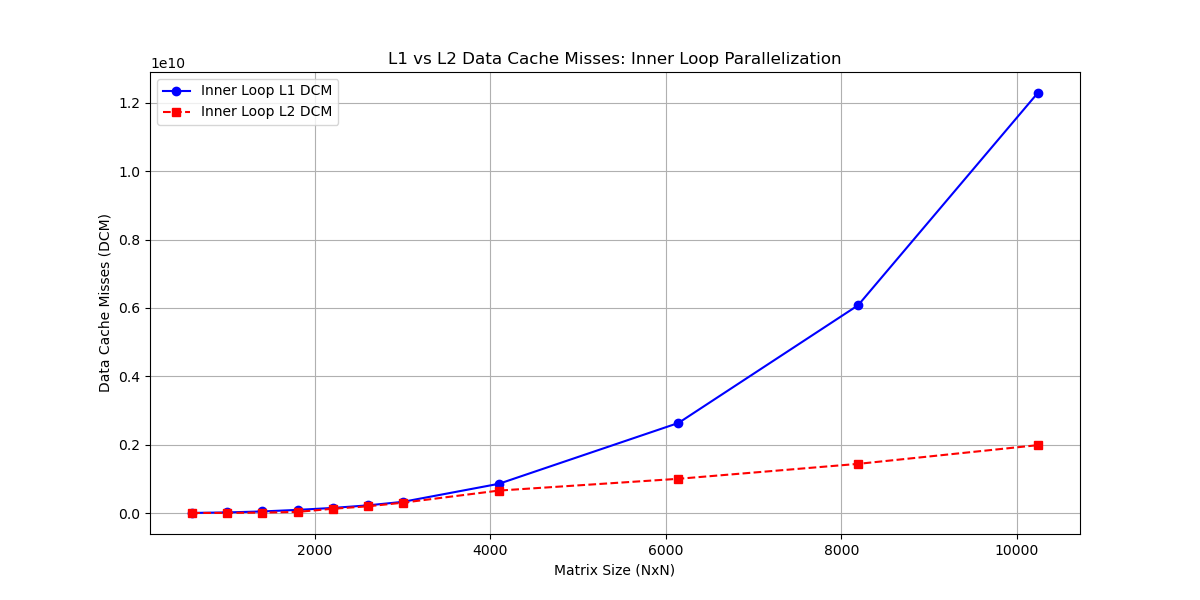
\includegraphics[width=\textwidth]{Figure_9.png} % Replace with your second image
        \caption{\small Inner Parallelization L1 vs L2 DCM Comparison}
        \label{fig:cache_misses_parallel2}
    \end{minipage}
    \hfill
    \begin{minipage}{0.48\textwidth} % Second row, second image
        \centering
        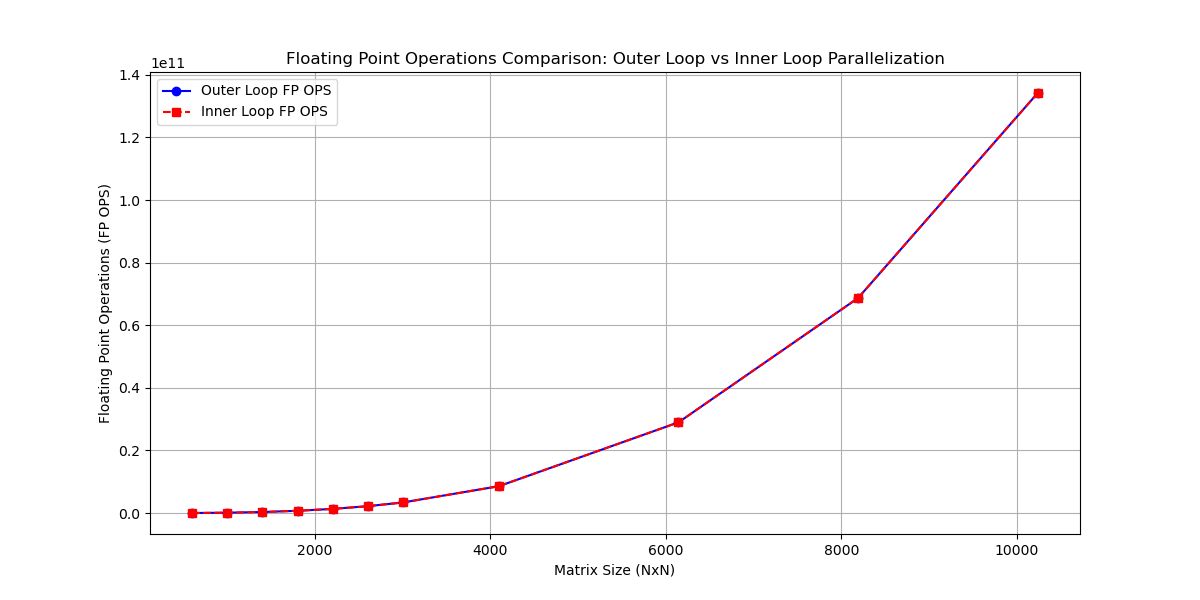
\includegraphics[width=\textwidth]{Figure_10.png} % Replace with your third image
        \caption{\small Parallel FP OPS Comparison}
        \label{fig:fp_ops}
    \end{minipage}

    \begin{minipage}{0.48\textwidth} % Third row, centered single image
        \centering
        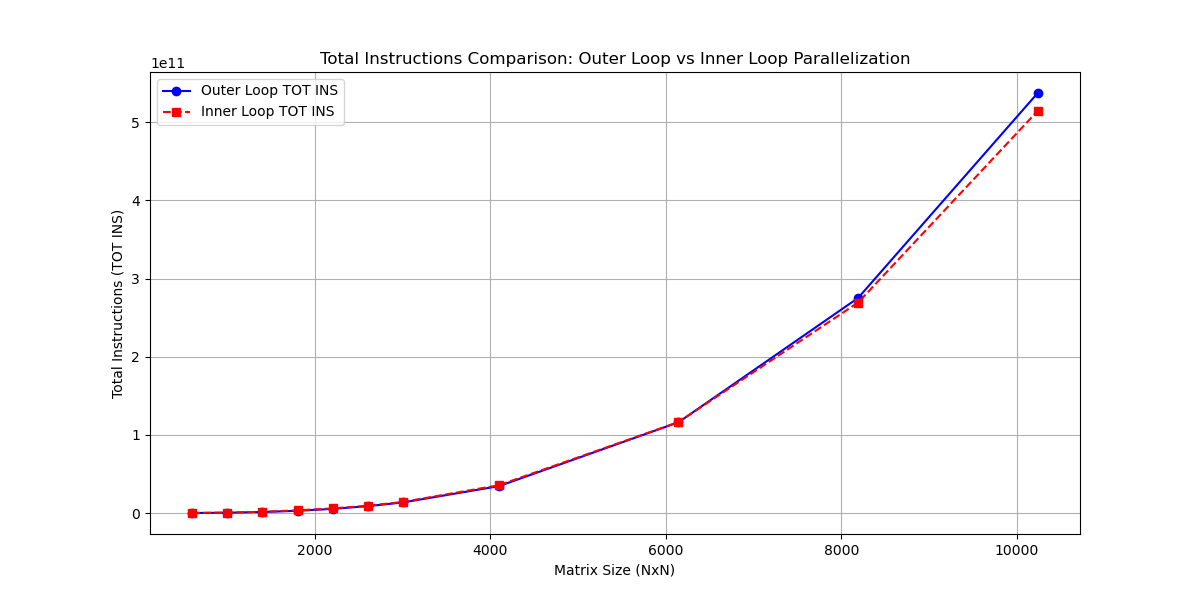
\includegraphics[width=\textwidth]{Figure_11.png} % Replace with your fourth image
        \caption{\small Parallel TOT INS Comparison}
        \label{fig:tot_ins}
    \end{minipage}
\end{figure}

After analyzing the execution time, cache performance, floating-point operations, and instruction count across different parallelization strategies, we can draw the following conclusions:


\textbf{Outer Loop Parallelization} is the better approach for larger matrix computations due to:

\begin{itemize}
    \item Faster execution time with lower computational overhead.
    \item Better cache efficiency, reducing L1 misses.
    \item Fewer floating-point operations and total instructions.
    \item Improved scalability with increasing matrix size.
\end{itemize}

\textbf{Inner Loop Parallelization} is less efficient for large matrices, leading to:

\begin{itemize}
    \item Higher cache misses and inefficient memory access.
    \item Increased synchronization overhead and poor scalability.
    \item Higher instruction count and computational redundancy.
\end{itemize}

\textbf{Verdict:} Outer loop parallelization is the preferred method for performance and scalability.

\section{Conclusions}


 \par The results highlighted the critical role of memory hierarchy and cache efficiency in computational performance.\par In single-core execution, C++ consistently outperformed Java for larger matrix sizes due to better memory management and lower runtime overhead. Java, on the other hand, leveraged JIT(Just In Time) optimizations to achieve better performance for smaller matrices. However, Java's efficiency dropped significantly as the matrix size increased due to higher memory overhead and garbage collection impacts. \par In multi-core execution, outer loop parallelization proved to be the more efficient strategy, offering better execution time, cache utilization, and computational efficiency. On the other hand, inner loop parallelization exhibited higher cache misses and synchronization overhead, making it less suitable for large-scale computations.\par Regarding block-oriented matrix multiplication, it did not scale well for larger matrices, with exponentially increasing execution times and suboptimal GFLOPS performance, primarily due to poor cache utilization. \par Overall, the findings emphasized that hardware-conscious optimizations are crucial for improving matrix multiplication performance. Additionally, choosing the right parallelization strategy is essential for maximizing efficiency, particularly when working with large datasets on modern multi-core processors.

\end{document}